% easychair.tex,v 3.5 2017/03/15

\documentclass{easychair}
%\documentclass[EPiC]{easychair}
%\documentclass[EPiCempty]{easychair}
%\documentclass[debug]{easychair}
%\documentclass[verbose]{easychair}
%\documentclass[notimes]{easychair}
%\documentclass[withtimes]{easychair}
%\documentclass[a4paper]{easychair}
%\documentclass[letterpaper]{easychair}
\usepackage{wrapfig}
\usepackage[font=small,labelfont=bf]{caption}

\usepackage{doc}
\usepackage{minted} % pip3 install pygments, pdflatex -shell-escape hb
\newminted[elpicode]{elpi.py:ElpiLexer -x}{linenos=true,fontsize=\footnotesize,escapeinside=\%\%}
\newmintinline[elpi]{elpi.py:ElpiLexer -x}{fontsize=\small}
\newminted[coqcode]{elpi.py:CoqElpiLexer -x}{firstnumber=last,linenos=true,fontsize=\footnotesize,mathescape,escapeinside=\#\#}
\newmintinline[coq]{elpi.py:CoqElpiLexer -x}{fontsize=\small}
\definecolor{dkgreen}{rgb}{0, 0.502, 0}
\bibliographystyle{plainurl}% the mandatory bibstyle

% use this if you have a long article and want to create an index
% \usepackage{makeidx}

% In order to save space or manage large tables or figures in a
% landcape-like text, you can use the rotating and pdflscape
% packages. Uncomment the desired from the below.
%
% \usepackage{rotating}
% \usepackage{pdflscape}

% Some of our commands for this guide.
%
\newcommand{\easychair}{\textsf{easychair}}
\newcommand{\miktex}{MiK{\TeX}}
\newcommand{\texniccenter}{{\TeX}nicCenter}
\newcommand{\makefile}{\texttt{Makefile}}
\newcommand{\latexeditor}{LEd}

%\makeindex

%% Front Matter
%%
% Regular title as in the article class.
%
\title{Hierarchy Builder}

% Authors are joined by \and. Their affiliations are given by \inst, which indexes
% into the list defined using \institute
%

\author{Cyril Cohen\inst{1} \and Kazuhiko Sakaguchi\inst{2} \and Enrico Tassi\inst{3}}

\institute{
 Inria, Universit\'e C\^ote d'Azur, France\\ \email{Cyril.Cohen@inria.fr}
\and
 University of Tsukuba, Japan\\ \email{sakaguchi@logic.cs.tsukuba.ac.jp}
\and
 Inria, Universit\'e C\^ote d'Azur, France\\\ \email{Enrico.Tassi@inria.fr}
}

%  \authorrunning{} has to be set for the shorter version of the authors' names;
% otherwise a warning will be rendered in the running heads. When processed by
% EasyChair, this command is mandatory: a document without \authorrunning
% will be rejected by EasyChair

\authorrunning{C.\,Cohen and K.\,Sakaguchi and E.\,Tassi}

% \titlerunning{} has to be set to either the main title or its shorter
% version for the running heads. When processed by
% EasyChair, this command is mandatory: a document without \titlerunning
% will be rejected by EasyChair
\titlerunning{Hierarchy Builder}
\newcommand{\HB}{\ensuremath{\mathcal{HB}}}

\begin{document}

\maketitle

%\begin{abstract}
%  We present a tool that makes it easy to build hierarchies
%  of algebraic structures in Coq.
%\end{abstract}

% The table of contents below is added for your convenience. Please do not use
% the table of contents if you are preparing your paper for publication in the
% EPiC Series or Kalpa Publications series

%\setcounter{tocdepth}{2}
%{\small
%\tableofcontents}

%\section{To mention}
%
%Processing in EasyChair - number of pages.
%
%Examples of how EasyChair processes papers. Caveats (replacement of EC
%class, errors).

\paragraph{Context and Talk proposal}

There is no questioning the importance of abstract algebra in the mathematical
vernacular. And it is with no surprise that libraries of machine checked code
are, nowadays, organized around hierarchies of structures. Unfortunately the
language of Type Theory and the features provided by the Coq system make the
construction of a hierarchy hard even for expert users. The difficulty
begins with the non-orthogonal choices of the encoding style, from bundled to
unbundled, and inference mechanism, from Type Classes to Canonical Structures.
To this, one may add the concerns about performance and about
the usability, by a non expert, of the final hierarchy.

In this talk we give an extensive demo of the Hierarchy Builder (\HB{})
extension for the Coq system version 8.10 and above.
\HB{} gives the library designer a language to describe the building blocks
of algebraic structures and to assemble them into a hierarchy. Similarly it
provides the final user linguistic constructs to build instances (examples) of
structures and to teach the elaborator of Coq how to take advantage of this
knowledge during type inference. Finally \HB{} lets the library designer
improve the usability of his library by providing alternative interfaces
to the primitive ones, a feature that can also be used to accommodate changes
to the hierarchy without breaking user code.

The details of \HB{}, including its compilation to the (Flat) Packed Classes
discipline and its implementation in the Elpi extension language for Coq,
are given in~\cite{cohen:hal-02478907}.
In this talk we focus on how to use \HB{} in a Coq development,
% and we plan to not detail how it works behind the scenes, 
unless questions on its internals arise from the audience.\\
\HB{} is available for download at \url{https://github.com/math-comp/hierarchy-builder}

\paragraph{Example: A hierarchy with a diamond in \HB{}}

\begin{coqcode}
HB.mixin Record CMonoid_of_Type A := { (* The set of axioms making A a commutative monoid. *)
  zero  : A;
  add   : A -> A -> A;
  addrA : associative add;  (* `add` is associative  *)
  addrC : commutative add;  (* `add` is commutative  *)
  add0r : left_id zero add; (* `zero` is the neutral *)
}.
HB.structure Definition CMonoid := { A of CMonoid_of_Type A }. (* The structure thereof. *)
Notation "0" := zero.
Infix    "+" := add.

(* The type of the operations and axioms depend on a CMonoid.type structure. *)
Check addrC. (* ?M : CMonoid.type |- forall x y : ?M, x + y = y + x *)

HB.mixin Record AbelianGrp_of_CMonoid A of CMonoid A := {
  (* We can write `add` here since A is a  CMonoid   *)
  opp   : A -> A;
  addNr : left_inverse zero opp add; (* `opp` is the additive inverse *)
}.
\end{coqcode}

\newpage

\begin{wrapfigure}[0]{r}{.35\textwidth}
  \vspace{1em}
  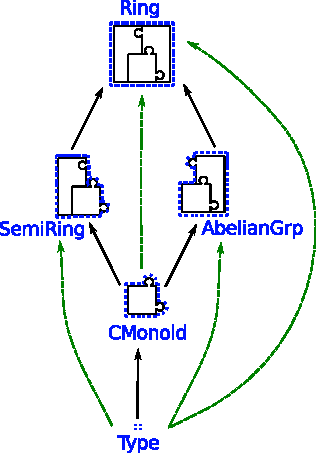
\includegraphics[width=.35\textwidth]{diagram.pdf}
  \vspace{-1.5em}
  \caption{The hierarchy}
  \label{fig:hierarchy}
\end{wrapfigure}
\
\begin{coqcode}
HB.structure Definition AbelianGrp := { A of AbelianGrp_of_CMonoid A & }.
Notation "- x"   := (opp x).
Notation "x - y" := (add x (opp y)).

(* A statement in the signature of an Abelian group G. *)
Check forall G : AbelianGrp.type, forall x : G, x - x = 0.

HB.mixin Record SemiRing_of_CMonoid A of CMonoid A := {
  one    : A;
  mul    : A -> A -> A;
  mulrA  : associative mul;  (* `mul` is associative   *)
  mul1r  : left_id one mul;  (* `one` is left neutral  *)
  mulr1  : right_id one mul; (* `one` is right neutral *)
  mulrDl : left_distributive mul add;  (* `mul` distributes over *)
  mulrDr : right_distributive mul add; (*   `add` on both sides  *)
  mul0r  : left_zero zero mul;  (* `zero` is absorbing `mul`     *)
  mulr0  : right_zero zero mul; (*   on both sides               *)
}.
HB.structure Definition SemiRing := { A of SemiRing_of_CMonoid A & }.
Notation "1"  := one.
Notation "-1" := (- one).
Infix    "*"  := mul.

(* A statement in the signature of a `SemiRing` S.  *)
Check forall S : SemiRing.type, forall x : S, x * 1 + 0 = x.

(* We need no additional mixin to declare the `Ring` structure. *)
HB.structure Definition Ring := { A of SemiRing_of_CMonoid A & AbelianGrp_of_CMonoid A }.

(* A statement in the signature of a Ring R.  *)
Check forall R : Ring.type, forall x : R, x * -1 = - x.

(* We equip Z with the structures of CMonoid, AbelianGrp and SemiRing; HB equips it with Ring. *)
Definition Z_CMonoid    := CMonoid_of_Type.Build Z 0%Z Z.add Z.add_assoc Z.add_comm Z.add_0_l.
HB.instance Z Z_CMonoid.
Definition Z_AbelianGrp := AbelianGrp_of_CMonoid.Build Z Z.opp Z.add_opp_diag_l.
HB.instance Z Z_AbelianGrp.
Definition Z_SemiRing   := SemiRing_of_CMonoid.Build Z 1%Z Z.mul Z.mul_assoc Z.mul_1_l ...
HB.instance Z Z_SemiRing.

(* A statement in the signature of the Z ring *)
Check forall x : Z, x * - (1 + x) = 0 + 1.
\end{coqcode}

For space constraints we omit the declaration
of the green arrows in Fig.~\ref{fig:hierarchy} which are alternative interfaces
called factories. They provide specialized interfaces to
build structures for others.
Factories are used to accommodate the insertion of
intermediate structures in a hierarchy without breaking user code, as we all
as to implement shortcuts: the factory to build a \coq{Ring} from \coq{Type}
(rightmost green arrow)
can omit the commutativity axiom of the addition, since it is implied
by the other axioms~\cite{nearrings}.
\bibliography{biblio}

\end{document}

%%% Local Variables:
%%% mode: latex
%%% TeX-master: "easychair.tex"
%%% TeX-command-extra-options: "-shell-escape"
%%% ispell-local-dictionary: "english"
%%% End: